\documentclass[14pt,a4paper]{extarticle}

\usepackage[utf8]{inputenc}
\usepackage[T2A]{fontenc}
\usepackage{amssymb,amsmath,mathrsfs,amsthm}
\usepackage[russian]{babel}
\usepackage{graphicx}
\usepackage[footnotesize]{caption2}
\usepackage{indentfirst}
\usepackage{multicol}
\usepackage{listings}
\usepackage{float}
\usepackage{url}
\usepackage{amsmath}

\usepackage{enumitem}

%\usepackage[ruled,section]{algorithm}
%\usepackage[noend]{algorithmic}
%\usepackage[all]{xy}
\usepackage{booktabs}
\usepackage{graphicx}
\usepackage[table,xcdraw]{xcolor}
\usepackage{tcolorbox}

%Библиотека для блок-схем
\usepackage{tikz}
\usetikzlibrary{shapes,arrows}

% Параметры страницы
\textheight=24cm
\textwidth=16cm
\oddsidemargin=5mm
\evensidemargin=-5mm
\marginparwidth=36pt
\topmargin=-1cm
\footnotesep=3ex
%\flushbottom
\raggedbottom
\tolerance 3000
% подавить эффект "висячих стpок"
\clubpenalty=10000
\widowpenalty=10000
%\renewcommand{\baselinestretch}{1.1}
\renewcommand{\baselinestretch}{1.5} %для печати с большим интервалом

\newcommand{\angstrom}{\mbox{\normalfont\AA}}

\newtheorem{definition}{Определение} % задаём выводимое слово (для определений)
\newtheorem{example}{Замечание} % задаём выводимое слово (для определений)
\newtheorem{theorem}{Теорема} % задаём выводимое слово (для определений)
\newtheorem{proposition}{Утверждение} % задаём выводимое слово (для определений)
\newtheorem{construction}{Конструкция} % задаём выводимое слово (для определений)

\DeclareMathOperator*{\sgn}{sgn}
\DeclareMathOperator*{\var}{var}
\DeclareMathOperator*{\cov}{cov}
\DeclareMathOperator*{\law}{Law}

\newcommand{\1}{\mathbbm{1}}
\newcommand{\R}{\mathbb{R}}
\newcommand{\N}{\mathbb{N}}
\newcommand{\Z}{\mathbb{Z}}
\renewcommand{\P}{\mathbb{P}}
\newcommand{\E}{\mathbb{E}}

\newcommand{\independent}{\perp\!\!\!\!\perp}

\newcommand\cA{{\cal A}}
\newcommand\cE{{\cal E}}
\newcommand\cC{{\cal C}}
\newcommand\cF{{\cal F}}
\newcommand\cG{{\cal G}}
\newcommand\cK{{\cal K}}
\newcommand\cL{{\cal L}}
\newcommand\cB{{\cal B}}
\newcommand\cN{{\cal N}}
\newcommand\cM{{\cal M}}
\newcommand\cX{{\cal X}}
\newcommand\cD{{\cal D}}
\newcommand\cR{{\cal R}}
\newcommand\cP{{\cal P}}
\newcommand\cQ{{\cal Q}}
\newcommand\cS{{\cal S}}
\newcommand\cT{{\cal T}}
\newcommand\cV{{\cal V}}
\newcommand\cZ{{\cal Z}}

\newcommand{\textProposition}    {Предложение}
\newcommand{\textTask}    {Задача}

\begin{document}

\begin{center}
    {Всеволод Заостровский, 409 группа}\\
    {\bfseries Отчёт по задаче ''Численное решение дифференциальных уравнений с частными производными. Нявная схема для уравнения теплопроводности''.\\}
    \vspace{1cm}
\end{center}

\section{Постановка задачи.} Необходимо решить уравнение:
\begin{equation} \label{diffeq1}
    u_t(t, x) = u_{xx}(t, x) - p(x) u(t, x) + f(t, x).
\end{equation}
В моём варианте, краевые условия:
\begin{equation} \label{diffeqedge}
    u(0, t) = 0, \quad u(1, t) = 0, \quad u(x, 0) = u_0(x). 
\end{equation}


\section{Решение дифференциального уравнения (для тестов).}\label{solution}
Будем искать решение в виде $u(t, x) = X(x) T(t)$. С учетом краевых условий, получим:
\begin{align*} 
    & u(0, x) = T(t) X(0) = 0 \Rightarrow X(0) = 0, \\
    & u(1, x) = T(t) X(1) = 0 \Rightarrow X(1) = 0.
\end{align*}
Разрешим уравнение с учетом $u(t, x) = X(x) T(t)$:
\begin{align*} 
    & X T' = X'' T, \\
    & \frac{X''}{X} = \frac{T'}{T} = -\lambda.
\end{align*}
Рассмотрим уравнение на $X$, чтобы найти значения $\lambda$, при которых решение нетривиально:
\begin{align*} 
    & X'' = -\lambda X, \\
    & X = C_1 \sin(\sqrt{\lambda} x) + C_2 \cos (\sqrt{\lambda} x), \\
    & X(0) = C_1 \sin(\sqrt{\lambda} 0) + C_2 \cos (\sqrt{\lambda} 0) = C_2 = 0 \Rightarrow C_2 = 0. \\
    & X(1) = C_1 \sin(\sqrt{\lambda} 1) + 0 * \cos (\sqrt{\lambda} 1)= 0 \Rightarrow \\ 
    & \Rightarrow \sin(\sqrt{\lambda}) = 0 \Rightarrow \sqrt{\lambda} = \pi k, k \in Z \Rightarrow \lambda = \pi^2 k^2, k \in Z.
\end{align*}
Случай $C_1 = 0$ дает тривиальное решение. С учетом вычислений выше, можем записать общий вид для $X$ и $T$:
\begin{align*} 
    & X = C_1 \sin(\pi k x), \quad T = C_2 \exp{(-\pi^2 k^2 t)}, \quad k \in Z.
\end{align*}
Таким образом, общее решение дифференциального уравнения:
\begin{align*} 
    & u = \sum_{n = 1}^{\infty} A_n \sin(\pi n x) \exp{(-\pi^2 n^2 t)}.
\end{align*}



\section{Дискретизация дифференциального уравнения.}
\begin{align} \label{scheme1}
    &\frac{u_m^{n+1} - u_m^n}{\tau} = \frac{u_{m+1}^{n+1} - 2 u_{m}^{n+1} + u_{m-1}^{n+1}}{h^2} - p(x_m) u_m^{n+1} + f(t_{n}, x_{m+1}),\\ 
    & m = 1 \ldots M-1, \\
    & n = 1 \ldots N-1. \\
\end{align}
В моём варианте, краевые условия:
\begin{equation} \label{schemeedge}
    \forall n, m: \quad u_0^{n} = 0, \quad u_1^{n} = 0, \quad u_m^{0} = u_0(x_m). 
\end{equation}
Заметим также, что существует схема Кранка--Николсона, формально дающая сходимость $O(h^2 + \tau^2)$. Однако, во-первых, задание требует неявную 
схему (а не полунеявную), а, во-вторых, такая сходимость недостижима в этой схеме практически из-за численных проблем.
\section{Аппроксимация на решении.}
Разложим значения решения в ряд Тейлора:

\begin{align*}
    u(t_n, x_{m+1}) &= u(t_n, x_{m}) +    h u_x(t_n, x_{m}) 
    + \frac{h^2}{2}u_{xx}(t_n, x_{m}) +    \frac{h^3}{6}u_{xxx}(t_n, x_{m}) \\ &+    \frac{h^4}{24}u_{xxxx}(t_n, x_{m}) + O(h^5) \\
    u(t_n, x_{m-1}) &= u(t_n, x_{m}) -    h u_x(t_n, x_{m}) 
    + \frac{h^2}{2}u_{xx}(t_n, x_{m}) -    \frac{h^3}{6}u_{xxx}(t_n, x_{m}) \\ &+    \frac{h^4}{24}u_{xxxx}(t_n, x_{m}) + O(h^5) \\
    u(t_{n+1}, x_m) &= u(t_{n}, x_m)+ \tau u_x(t_{n}, x_m) + \frac{\tau^2}{2}u_{tt}(t_n, x_{m}) + \frac{\tau^3}{6}u_{ttt}(t_n, x_{m}) \\
    &+ \frac{\tau^4}{24}u_{tttt}(t_n, x_{m}) + O(\tau^5) \\
    u(t_{n-1}, x_m) &= u(t_{n}, x_m)- \tau u_x(t_{n}, x_m) + \frac{\tau^2}{2}u_{tt}(t_n, x_{m}) - \frac{\tau^3}{6}u_{ttt}(t_n, x_{m}) \\
    &+ \frac{\tau^4}{24}u_{tttt}(t_n, x_{m}) + O(\tau^5) \\
\end{align*}
Отсюда имеем:
\begin{align*}
    \frac{u_m^{n+1} - u_m^n}{\tau} &=   \frac{u(t_{n+1}, x_m) - u(t_n, x_m)}{\tau} = u_t(t_{n}, x_m) \\
    &+\frac{\tau}{2}u_{tt}(t_n, x_{m}) + \frac{\tau^2}{6}u_{ttt}(t_n, x_{m}) + \frac{\tau^3}{24}u_{tttt}(t_n, x_{m}) + O(\tau^4) \\
    \frac{u_{m+1}^{n+1} - 2 u_{m}^{n+1} + u_{m-1}^{n+1}}{h^2} &= \frac{u(t_{n+1}, x_{m+1}) - 2 u(t_{n+1}, x_{m}) + u(t_{n+1}, x_{m-1})}{h^2} = \\
    &= u_{xx}(t_n, x_{m}) + \frac{h^2}{12}u_{xxxx}(t_n, x_{m}) + O(h^4)\\
\end{align*}

Подставив эти выражения в дифференциальное уравнение, получим:
\begin{align*}
    &||\frac{u_m^{n+1} - u_m^n}{\tau} - \frac{u_{m+1}^{n+1} + 2 u_{m}^{n+1} + u_{m-1}^{n+1}}{h^2} + p(x_m) u_m^{n+1} - f(t_{n}, x_{m+1})|| = \\
    &= ||- u_{xx}(t_n, x_{m}) + O(h^2) + u_t(t_{n}, x_m) + O(\tau) + p(x_m) u_m^{n+1} - f(t_{n}, x_{m+1}) || =\\
    &= O(h^2 + \tau). \\
\end{align*}
С учетом того, что начальные условия даны точно и, очевидно, $|f(t_n, x_m) - f_m^n| \rightarrow 0$, получаем, что порядок аппроксимации на решении 
данной схемы составляет $O(\tau + h^2)$.



\section{Устойчивость схемы.}
Удобная для анализа форма записи схемы имеет вид:
\begin{align*}
    u_m^{n+1} - u_m^n = \rho (u_{m+1}^{n+1} - 2 u_{m}^{n+1} + u_{m-1}^{n+1}) - \tau p(x_m) u_m^{n+1} + \tau f(t_{n}, x_{m+1}), \quad \rho = \frac{\tau}{h^2}.
\end{align*}

Выбирая из всех значений $u_m^{n+1}$, по модулю равных $\left\|u^{n+1}\right\|$, такое, у которого индекс $m$ принимает наименьшее значение, имеем
$$
\left|u_m^{n+1}\right|>\left|u_{m-1}^{n+1}\right| \text { и }\left|u_m^{n+1}\right| \geqslant\left|u_{m+1}^{n+1}\right| .
$$
Отсюда $\left|2 u_m^{n+1}\right|>\left|u_{m-1}^{n+1}\right|+\left|u_{m+1}^{n+1}\right|$, и знак выражения $2 u_m^{n+1}-u_{m-1}^{n+1}-u_{m+1}^{n+1}$ совпадает со знаком $u_m^{n+1}$, т. е. справедлива оценка снизу
$$
\left\|u^{n+1}\right\|=\left|u_m^{n+1}\right| \leq \left|u_m^{n+1}+\rho\left(2 u_m^{n+1}-u_{m-1}^{n+1}-u_{m+1}^{n+1}\right)\right|=\left|u_m^n+\tau f_m^{n+1}\right| .
$$
Таким образом, при любых шагах сетки $\tau$ и $h$ справедливо неравенство $\left\|u^{n+1}\right\| \leq \left\|u^n\right\|+\tau\left\|f^{n+1}\right\|$. Из него 
получаем:

$\begin{aligned}\left\|u^{n+1}\right\| & \leq \left\|u^n\right\| +\tau\left\|f^n\right\| 
     \leq \left\|u^{n-1}\right\|+\tau\left(\left\|f^n\right\|+\left\|f^{n-1}\right\|\right) 
    \leq  \ldots \leq \\ &\leq \left\|u^0\right\|+\sum_{k=0}^n \tau\left\|f^k\right\|
    \leq \left\|u^0\right\|+(n+1) \tau \max _k\left\|f^k\right\| .\end{aligned}$

Таким образом, схема бехусловно устойчива.

\section{Алгоритм построения сети.}
Отсюда имеем:
\begin{equation*} \label{scheme1}
    -\frac{u_{m+1}^{n+1}}{h^2} + u_m^{n+1} (\frac{1}{\tau} 
    + \frac{2}{h^2} + p(x_m)) - \frac{u_{m-1}^{n+1}}{h^2} = f(t_{n}, x_{m+1}) + \frac{u_m^n}{\tau}.
\end{equation*}

Фактически, требуется построить значения функции на сети. Процесс построения описывается рисунком \ref{scheme}: 
известны значения в левой, правой и нижней границах квадрата $[0,1] \times [0, 1]$. Значение в каждом узле определяется
значениями соседних узлов: слева, справа и непосредственно под ним. 

\begin{figure}
    \centering
    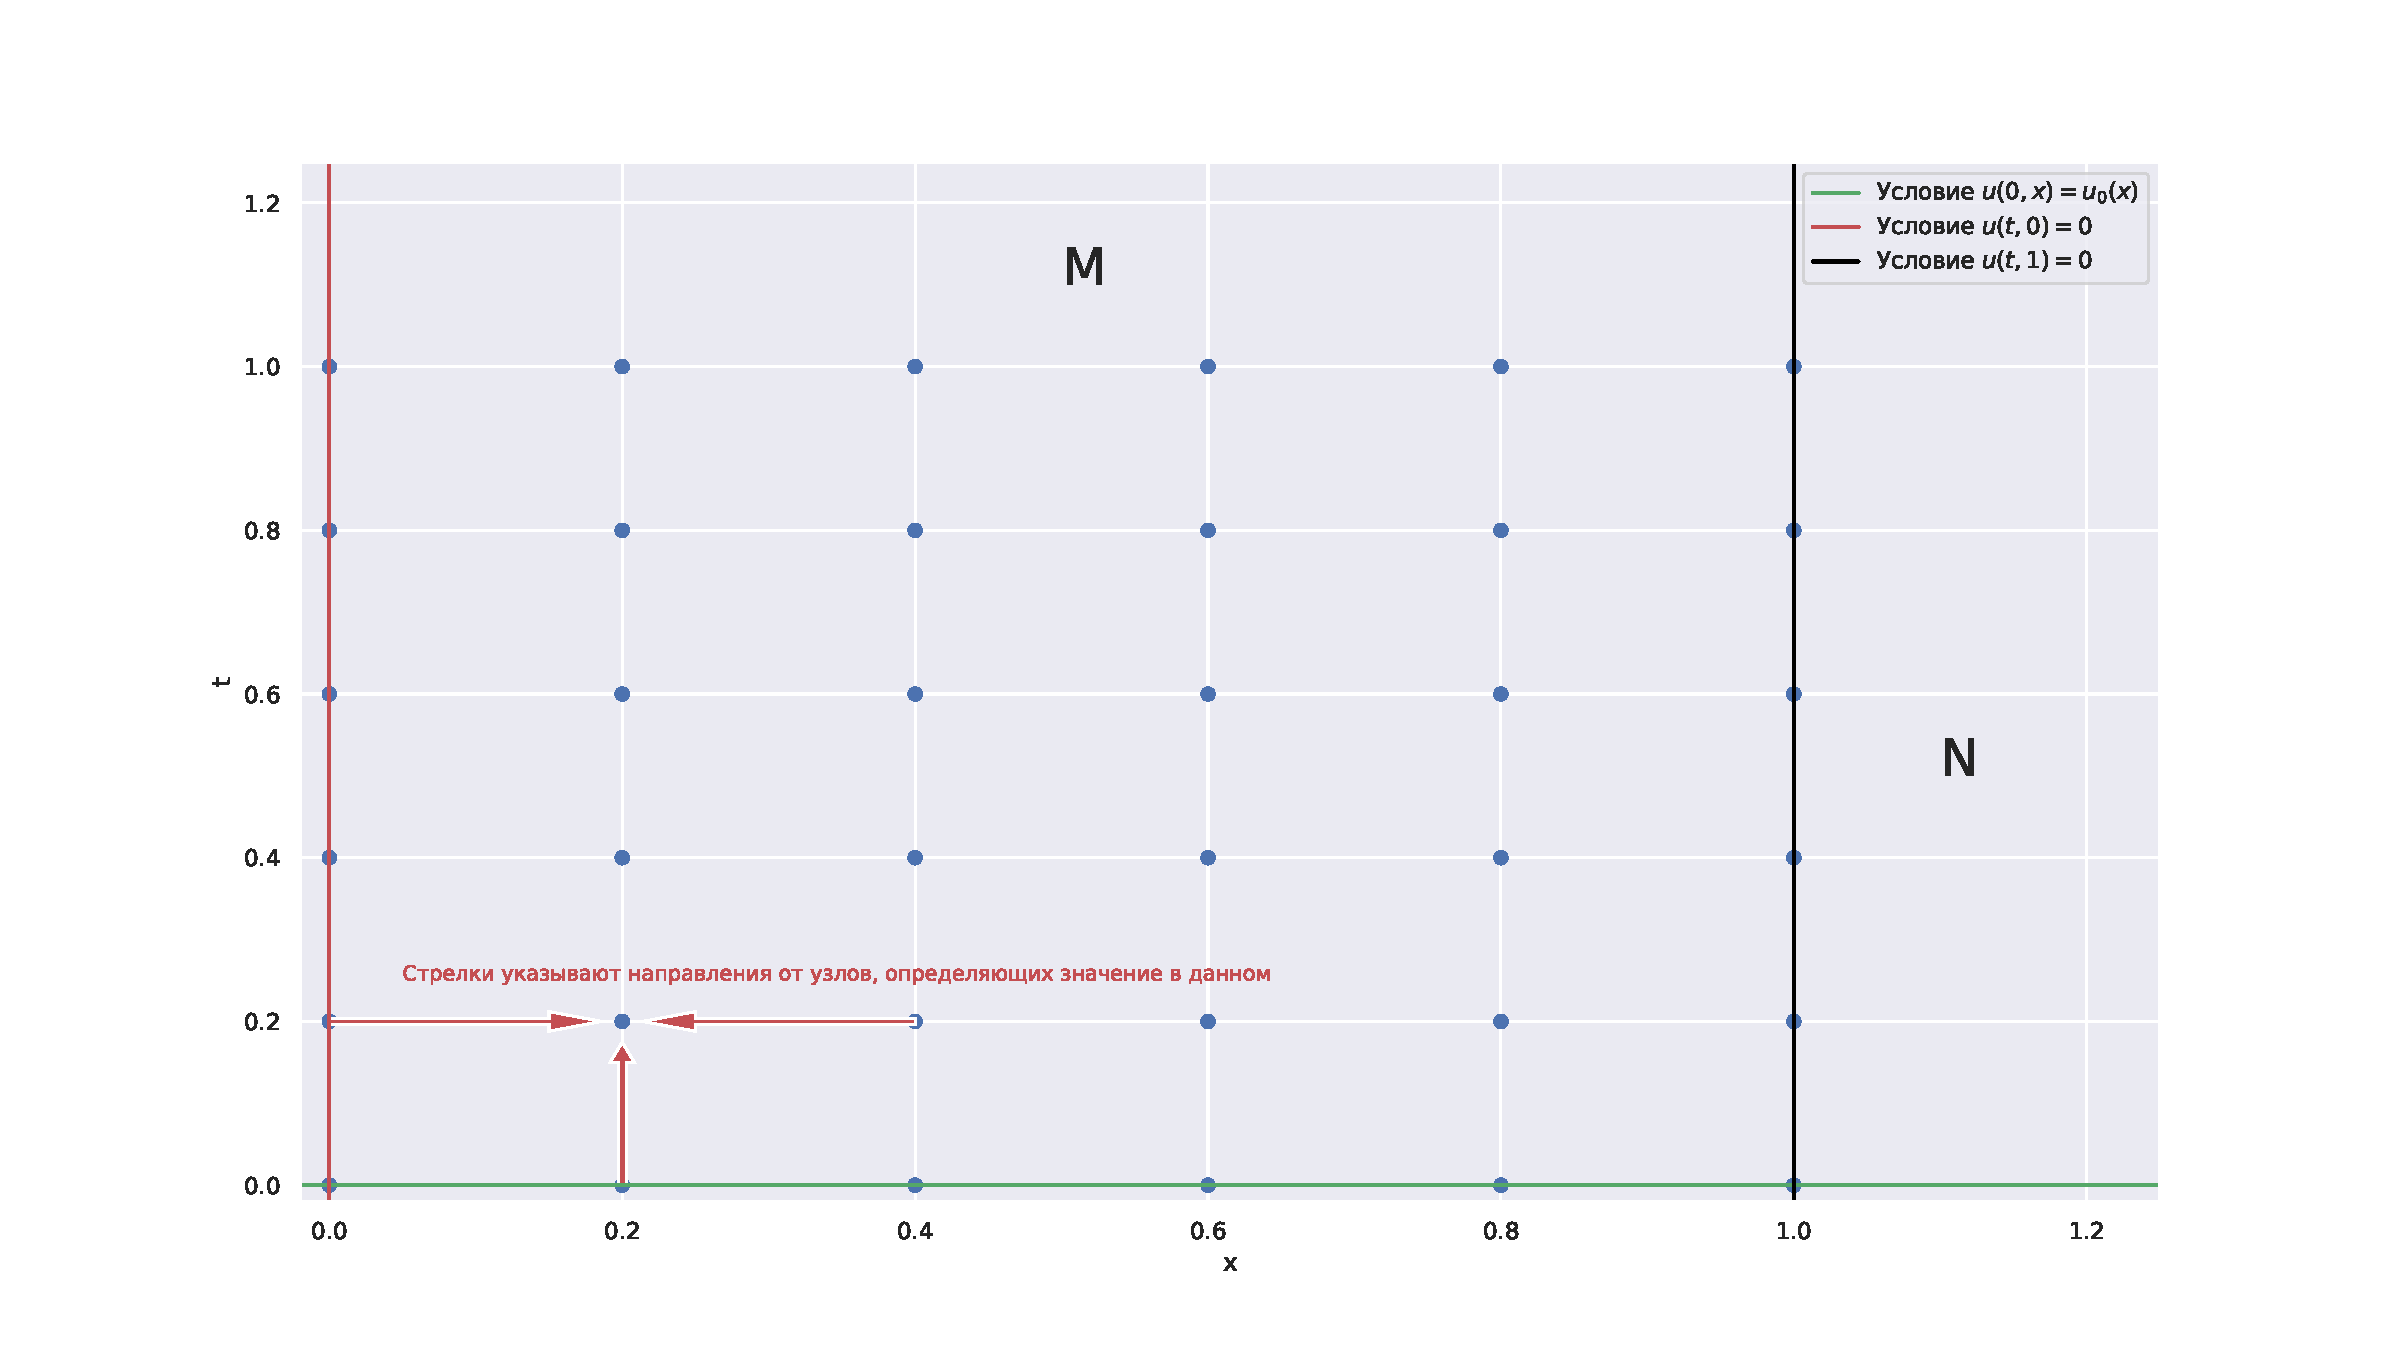
\includegraphics[scale=0.4]{figs/scheme.pdf}
    \caption{Графическое представление задачи и порядка вычисления значений в узлах сетки}
    \label{scheme}
\end{figure}

Таким образом, зная вектор $\{u_m^n\}_{m = 1, \ldots N-1}$ для нахождения вектора $\{u_m^{n+1}\}_{m = 1, \ldots M-1}$ необходимо решить систему:

$F = \begin{pmatrix}
    \frac{1}{\tau} + \frac{2}{h^2} + p(x_m)  &   -\frac{1}{h^2}                           & 0               & \ldots & 0 \\
    -\frac{1}{h^2}                           &   \frac{1}{\tau} + \frac{2}{h^2} + p(x_m)  & -\frac{1}{h^2}  & \ldots & 0  \\
    % 0  &-\frac{1}{h^2}  &   \frac{1}{\tau} + \frac{2}{h^2} + p(x_m)  & -\frac{1}{h^2} & \ldots & 0 \\
    \ldots  &\ldots  &   \ldots  & \ldots  & \ldots \\
    0 & \ldots & \ldots & 0 -\frac{1}{h^2}  &   \frac{1}{\tau} + \frac{2}{h^2} + p(x_m) 
\end{pmatrix}
\begin{pmatrix}
    u_1^{n + 1} \\
    u_2^{n + 1} \\
    \ldots \\
    u_{M-2}^{n+1} \\
    u_{M-1}^{n+1}
\end{pmatrix}$, 
где

$F=
\begin{pmatrix}
    f(t_{1}, x_{m+1}) + \frac{u_1^{n}}{\tau} \\
    f(t_{2}, x_{m+1}) + \frac{u_2^{n}}{\tau} \\
    \ldots \\
    f(t_{n-2}, x_{m+1}) + \frac{u_{M-2}^{n}}{\tau} \\
    f(t_{n-1}, x_{m+1}) + \frac{u_{M-1}^{n}}{\tau}
\end{pmatrix}$.


Сделать это можно, к примеру, методом прогонки.

\section{Тесты}
В разделе \ref{solution} найдено представление решения в виде ряда, коэффициенты которого определяются из условия $u(x, 0) = u_0(x)$. 
Для тестов возьмём  
$$u_0(x) = u(x,0)=\sin(\pi n x) .$$ 
В этом случае легко видеть из разложения общего решения в ряд, что
$$ u(t, x) = \sin(\pi x) \exp{(-\pi^2 t)}. $$
Было проведено два теста скорости сходимости: 
\begin{enumerate}
    \item $(N, M) = \left\{(i, i), \quad i \in \{100, 200, 300, 400, 500\} \right\}$ --- для проверки сходимоти $O(\tau)$.
    \item $(N, M) = \left\{(i^2, i), \quad i \in \{10, 20, 30\} \right\}$ --- для проверки сходимоти $O(h^2)$.
\end{enumerate}
Если $\delta(N, M) = \max_{n\leq N, m \leq M} |u(t_n, x_m) - u_h(t_n, x_m)| = O(h^2 + \tau), $ то: 
\begin{enumerate}
    \item при хорошем $h$ (в тесте взято $h = \tau  $): $ \ln\left(\delta(N, M)\right) \approx \ln(\tau) + \text{const},$
    \item при плохом  $h$ (в тесте взято $h = \sqrt{\tau}$): $ \ln\left(\delta(N, M)\right) \approx \ln(h) + \text{const}.$
\end{enumerate}
Из графиков \ref{t1} и \ref{t2} видно, что эти условия выполнены. 

\begin{figure}
    \centering
    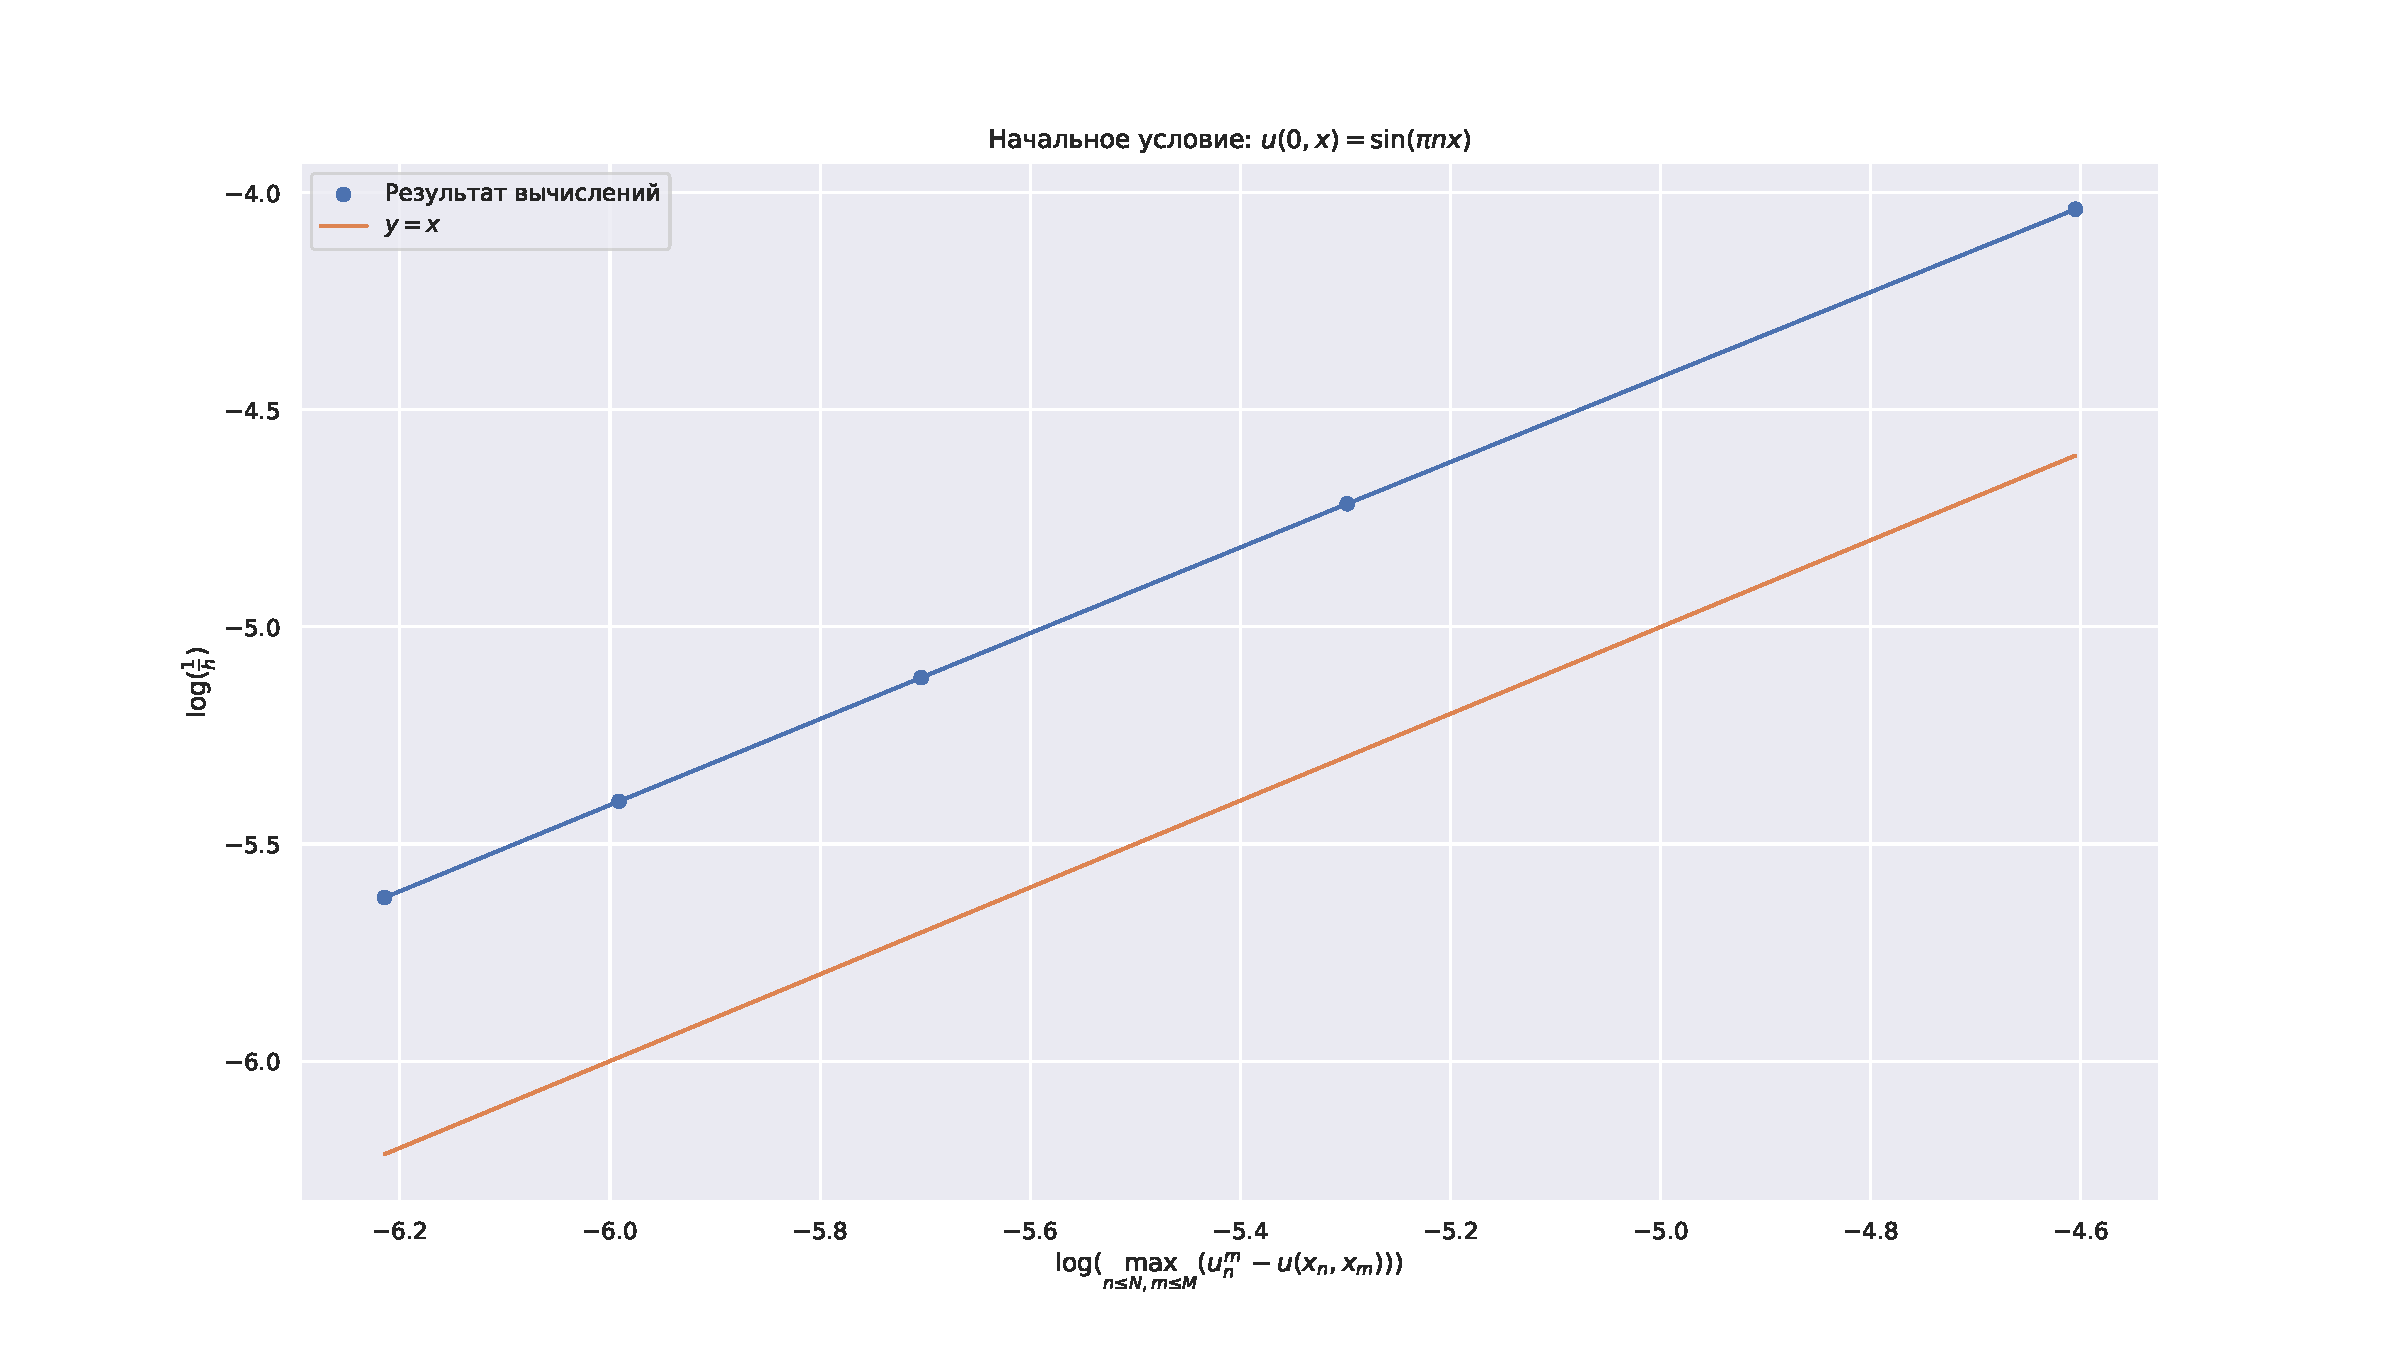
\includegraphics[scale=0.4]{figs/OrderCon1.pdf}
    \caption{Зависимость погрешности от размера сетки в первой серии тестов}
    \label{t1}
\end{figure}

\begin{figure}
    \centering
    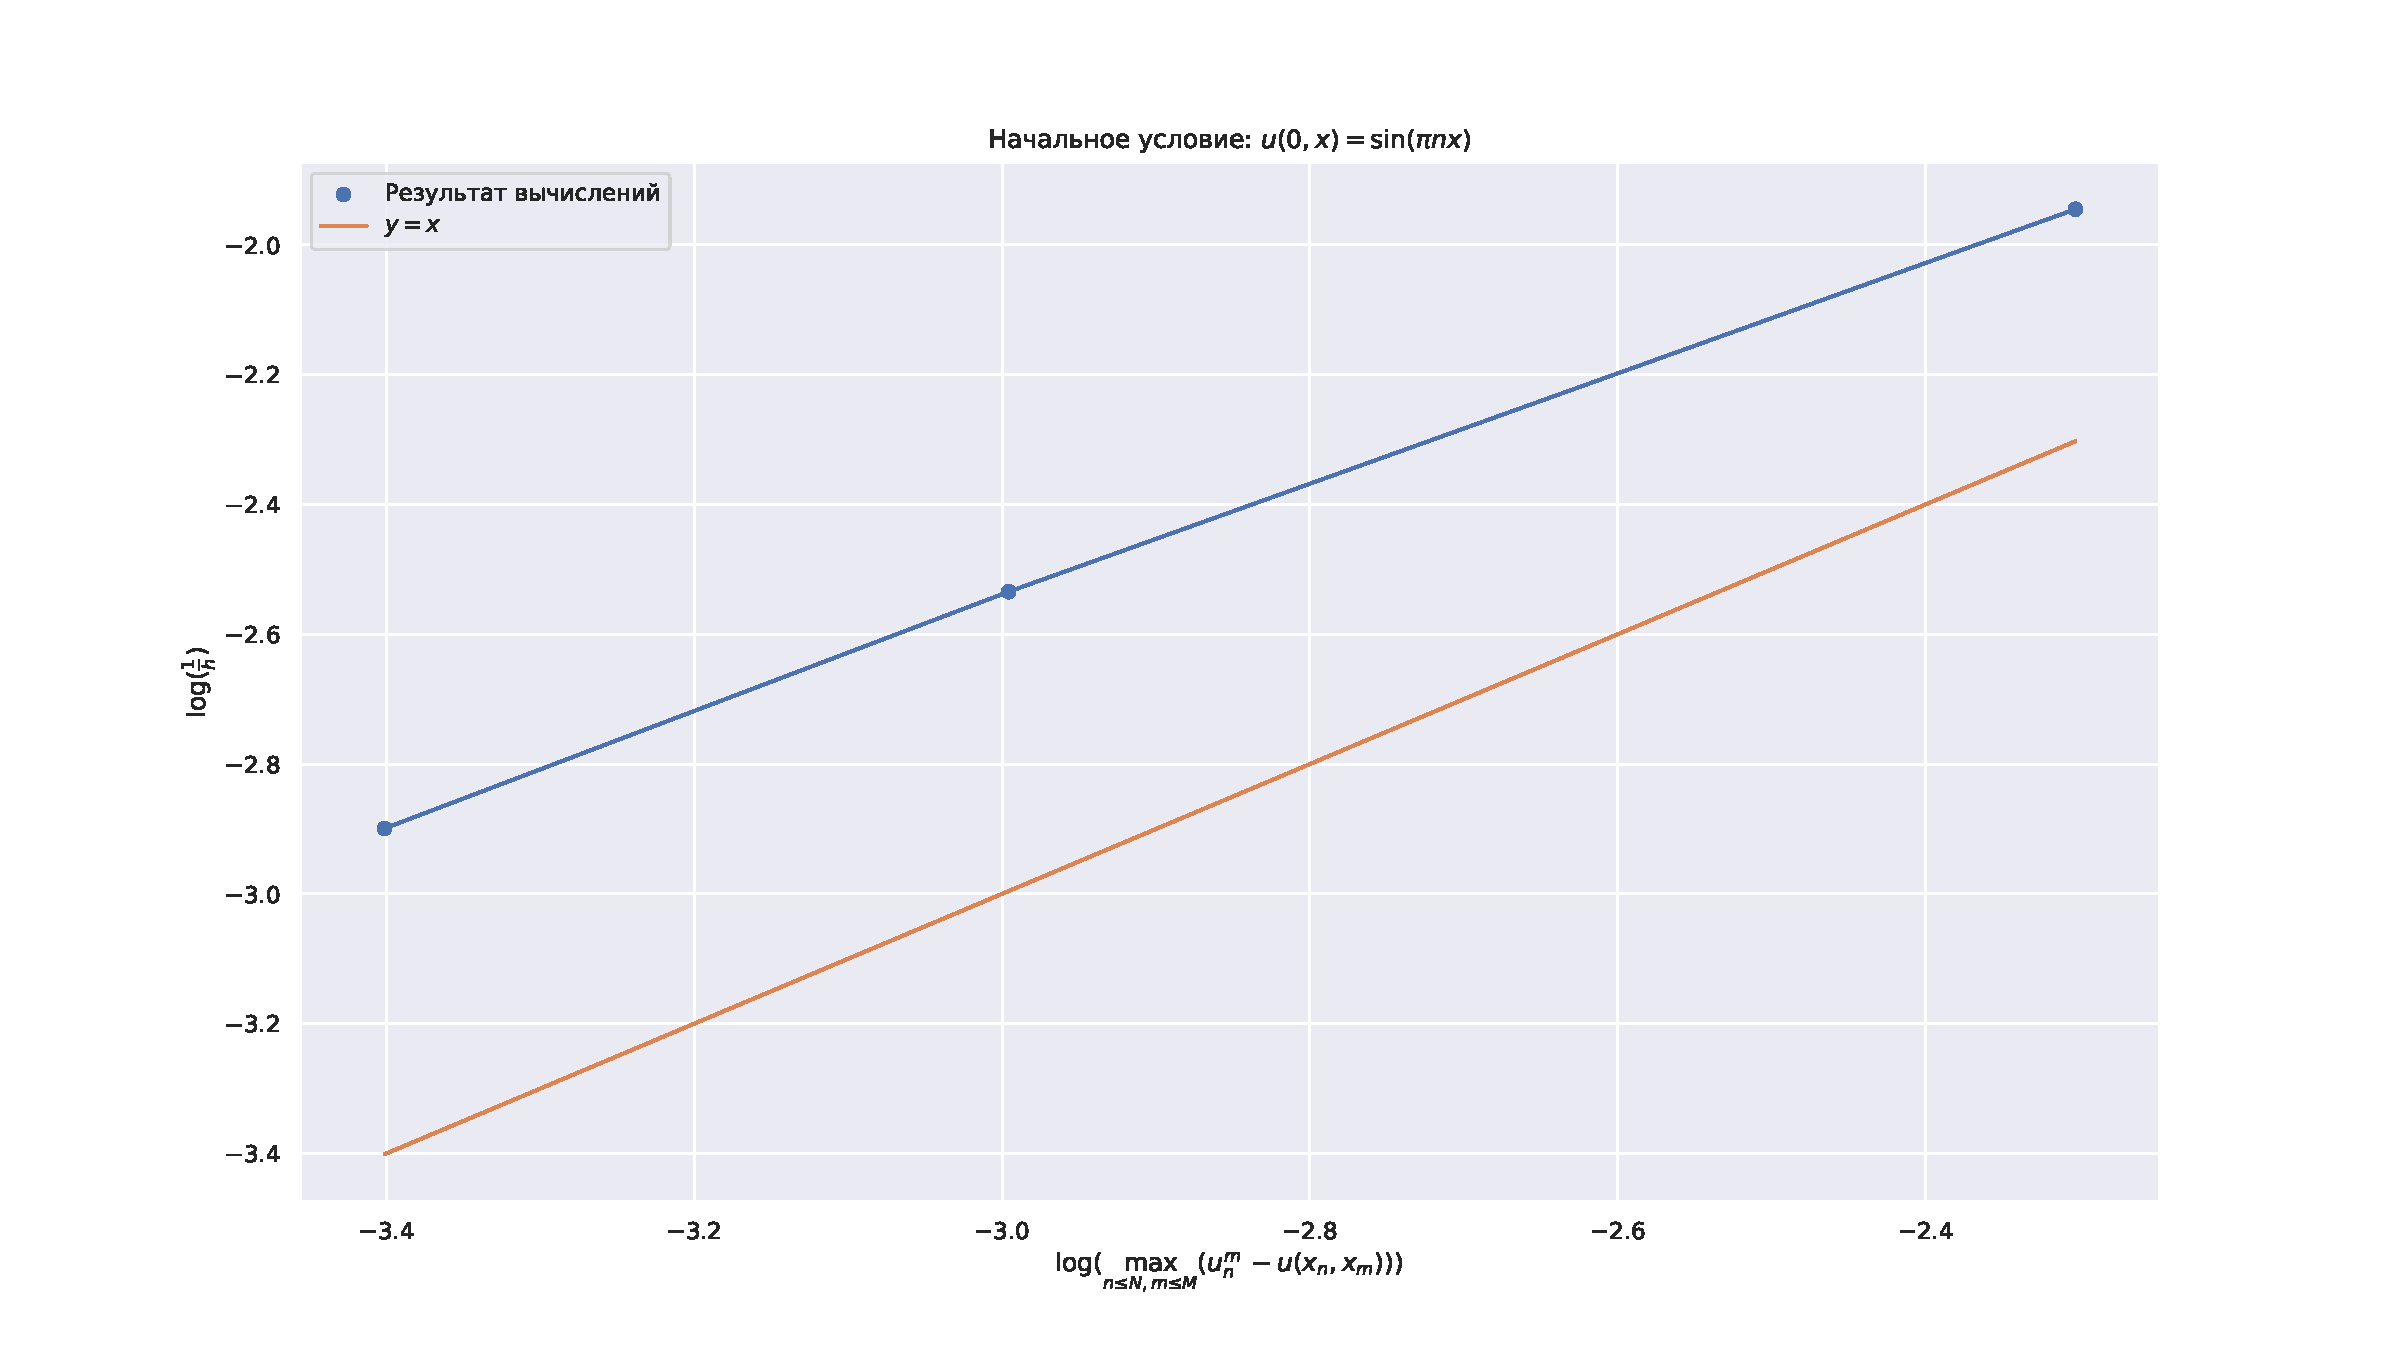
\includegraphics[scale=0.4]{figs/OrderCon2.pdf}
    \caption{Зависимость погрешности от размера сетки во второй серии тестов}
    \label{t2}
\end{figure}

\begin{figure}
    \centering
    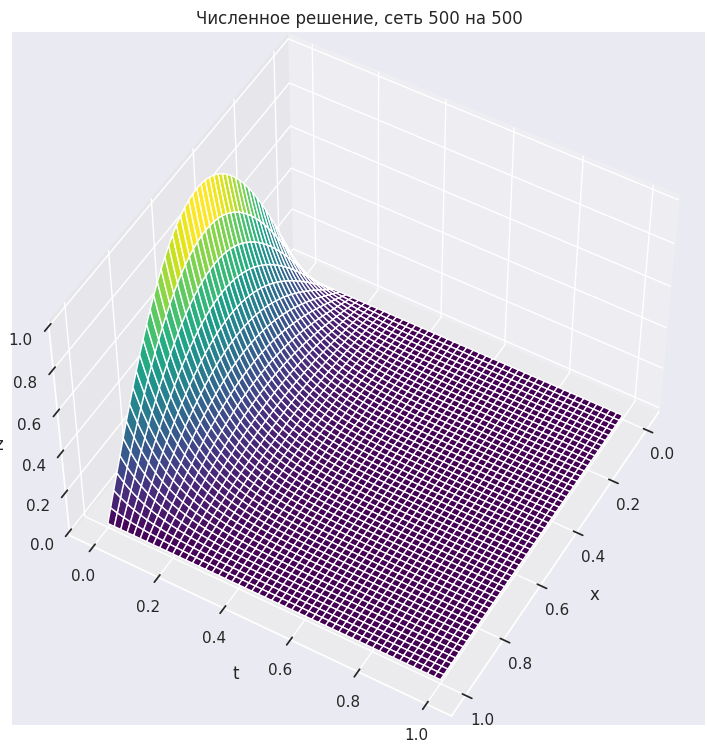
\includegraphics[scale=0.6]{figs/p500500.png}
\end{figure}

\begin{figure}
    \centering
    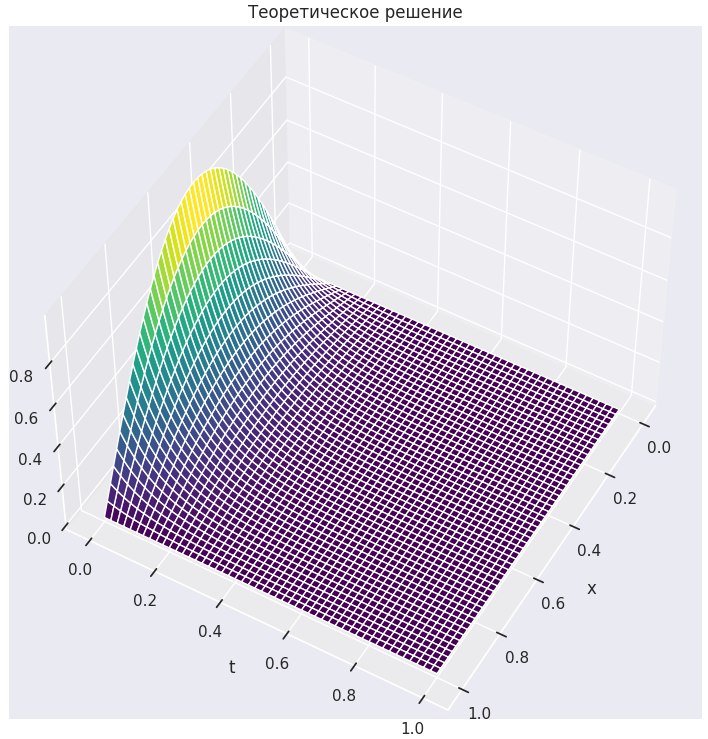
\includegraphics[scale=0.6]{figs/TeorSol.png}
\end{figure}

\begin{figure}
    \centering
    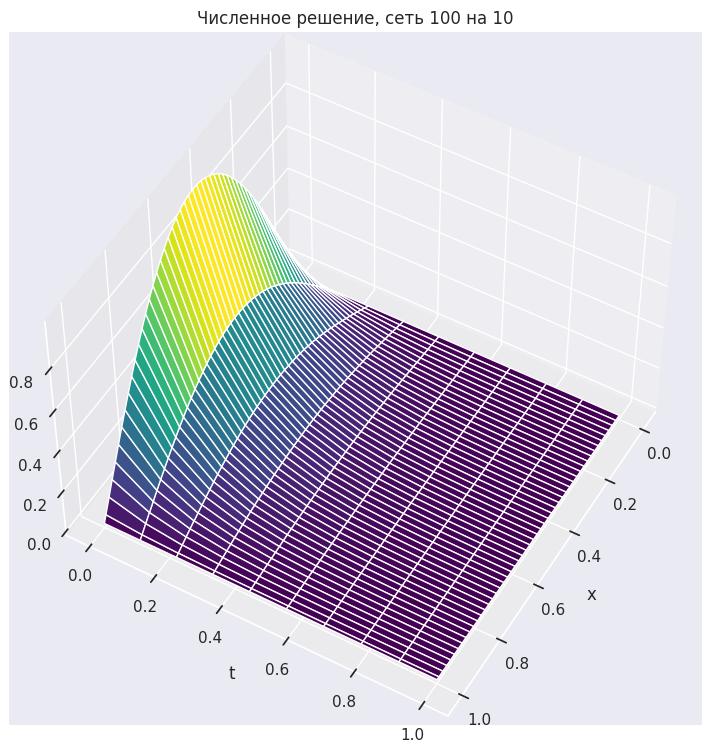
\includegraphics[scale=0.6]{figs/t10010.png}
\end{figure}

\end{document}